\documentclass[conference]{IEEEtran}
\IEEEoverridecommandlockouts
% The preceding line is only needed to identify funding in the first footnote. If that is unneeded, please comment it out.
\usepackage{cite}
\usepackage{amsmath,amssymb,amsfonts}
\usepackage{algorithmic}
\usepackage{graphicx}
\usepackage{textcomp}
\usepackage{xcolor}
\def\BibTeX{{\rm B\kern-.05em{\sc i\kern-.025em b}\kern-.08em
    T\kern-.1667em\lower.7ex\hbox{E}\kern-.125emX}}
\begin{document}

%THIS IS FOR THE TITLE 
\title{ \qquad\qquad Noam Chomsky and\newline The Linguistic Theory\\
{\footnotesize Written by Daniel Quiroga -- CSci 423W Assignment%\textsuperscript{*}Note: Sub-titles are not captured in Xplore and
%should not be used
}
\thanks{College of William and Mary - Daniel Quiroga - Computer Science}
}



\maketitle

\begin{abstract}
This Paper will summarize the life of Avram Noam Chomsky (I will refer to him as Noam Chomsky throughout the paper) and his theory of Linguisitics. It will dive into his upbringing and the path he took to become a massive contributor to Computational Theory. His Linguistic Theory has had major impacts on advancement in Computational Theories and allowed for more discoveries to arise. How his linguistic theory has an implication in more than just linguistics. 
\end{abstract}

\section{Life}
First and foremost, Noam Chomsky was born on December 7th, 1928 in Philadelphia, Pennsylvania, United States and is still alive today.\newline

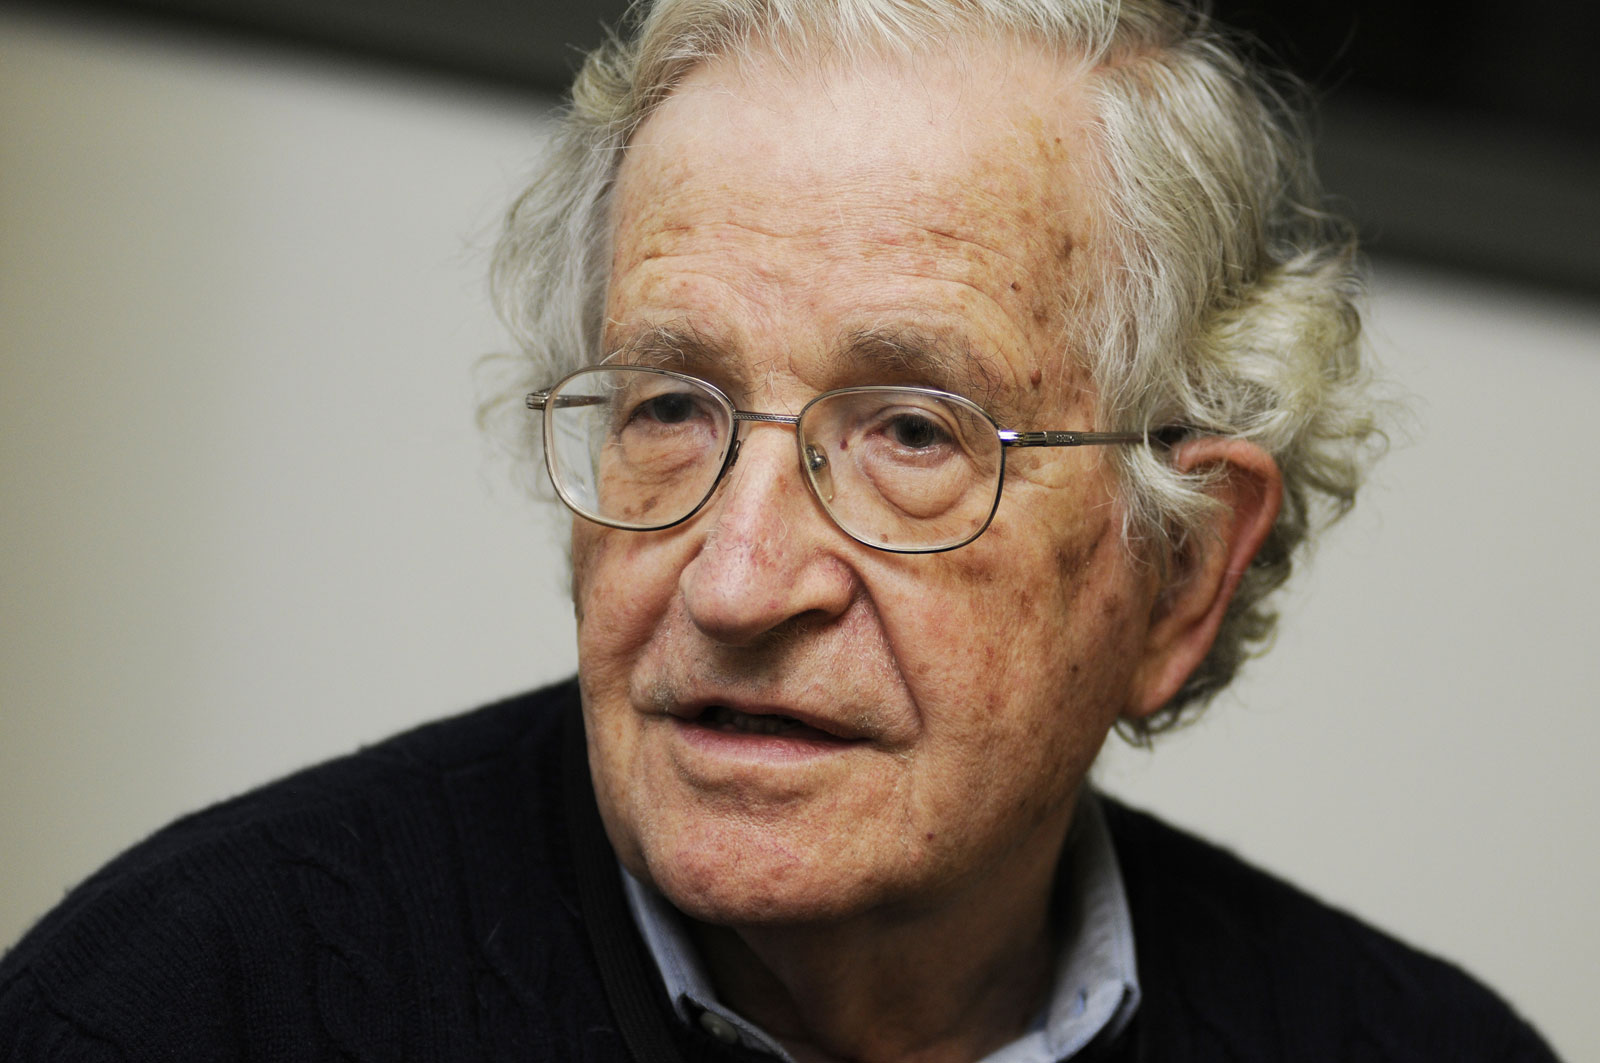
\includegraphics[scale=.1]{headshot.jpg} 

Photo 1: A headshot of Noam Chomsky

\subsection{Childhood}
On December 7th, 1928, Noam Chomsky was born in the East Oak Lane neighborhood in Philly. Both of his parents, Ze'ev Chomsky and Elsie Simonofsky, were Jewish immigrants[6]. 

Ze'ev fled, what was known as the Russian Empire, in the early 1900's to Baltimore, Maryland. He worked in various jobs and also local Hebrew elementary schools before pursuing higher education. Eventually, he moved to Philadelphia and began to work in a school centered around religion, which is where he met Noam's mother Elsie, where he was the principal. While at the head of the school, his philosophy was to have be people, "well integrated, free and independent in their thinking, concerned about improving and enhancing the world, and eager to participate in making life more menaingful and worthwhile for all"[6].

This was the ideology that Noam Chomsky adopted and carried forth his father's legacy. Noam's Mother Elsie was born in Belarus and was a teacher at the school that Ze'ev was the principal[6].

Noam is the firstborn, he has a younger brother, David Eli, that is a few years younger. They were very close growing up, but polar opposites. Noam was always very fierce while Eli was more calm. They both were raised with proper Jewish backgrounds and grew up learning the Hebrew Langugage. They sided with mostly Left Zionism and felt the repricushions in antisemitism from other relgious groups in Philly at the time. 

His education consisted of Philly's Central High School and Gratz College, the Hebrew High school where Ze'ev worked. He was always excellent academically and was involved in many different extracurriculars. 

Noam Chomsky said that both of his parents were moderate Democrats, but what mostly influenced him were other family members who were much more left in the political spectrum, boaderlining Socialism. Because of this Chomsky's first article, which he wrote at 10 years of age, was mainly about Facisim during the Spanish Civil War[1]. His later articles made a 'lucky accident' for condeming what Joeseph Stalin was doing and other forms of Marxism[6]. \newline


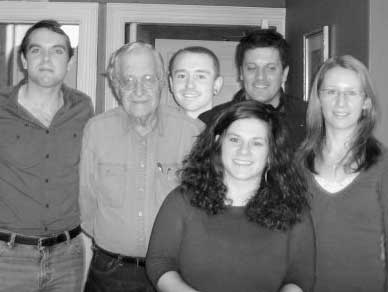
\includegraphics[scale=.5]{family.jpg} 

Photo 2: Noam and his family
\subsection{Higher Level Education}
At age 16, Noam Chomsky began his education at the University of Pennsylvania. He was undecided on what to study at first so he looked into logic, languages and philosophy. He paid for his education by teaching Hebrew and also saved lots of money by living with his parents, since he was still in Pennsylvania.

Chomsky was very close to dropping out of school and relocating to Palestine. The event that altered his time in higher education and eventually led to the Linguistic Theory (which I will discuss later in the Paper) was meeting linguist Zellig Harris, whom was also in his political circle (Coincidence?). Zellig was the person to revealed and ultimately influenced Noam to major in theoretical linguistics. The two thesis that Noam Chomsky wrote for his BA Honors and MA were heavily influence by Zellig Harris. His MA thesis was so good that eventually it was converted into a book. 

Later on, Chomsky attended Harvard where he began his PhD thesis. Chomsky chose Harvard due to the resources that were available to him there in the form of two excellent and over acheiving professors (D. Elliot and M. Ethan). He was impacted heavily by the two and eventually published Systems of Syntactic Analysis, which was apart of the Journal of Symbolic Logic. Although this was not in a journal for linguistic, he had lots of aspects in the field that appeared his the acadamic publishing. His first solid Linguistic piece came in 1955 when he turned in a thesis that consisted of what he thought of transformational grammer, where he was awarded a Doctor of Philosophy degree. This was eventually mulled and then published in The logical Structure of Linguistic Theory. Afterwards, he had some professors reach out to help structure other technical papers which included one in mathematical linguistics.

While his time at Harvard, Noam Chomsky met Carol Doris Schatz, whom was a childhood friend. They began a romantic relationship soon after he arrived at Harvard and eventually got married. When his time at Harvard finished, they relocated to an area inside of Boston, Massachusetts where they lived for the better part of a decade. After, they moved to a suburb in Lexington. They both recieved a grant by Harvard to travel most of Europe together. While on the trip, the presence of Jewish nationalism, anti-Arab racism caught Noam Chomsky's attention. 

Chomsky was very interested in politics. During many of his trips he would look to learn more and expand his knowledge of various ideologies. He was especially intersted in ideologies about anarchist and classical liberalism, which can be seen was influenced early on by his relatives. Due to his knowledge of a diverse number of ideologies, Chomsky began to create his own opinions and which he sided with the most was a anarcho-syndicalist society, specifically those that arose after the Spanish Civil War[1]. Another one that he really connected with was that of Marlentie ideas of an anti-Marxist community which had a point of view that WW2 was manipulated by capitalisms in the West and Soviet's to eliminate European proletariat [3]. \newline

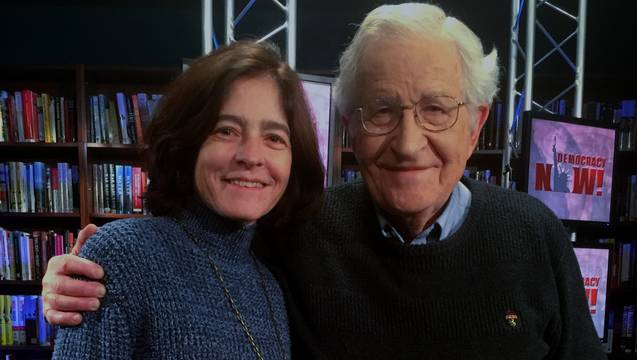
\includegraphics[scale=.25]{wife.jpg} 

Photo 3: of Noam and his wife
\subsection{Post-Graduate/Adult life}

Chomsky was able to get a job in a mechanical translation project and also as a teacher, teaching a course on linguistics and philosophy, in the Massachusetts Institude of Technology. He really enjoyed the Massachusetts Institude of Technology because of how liberal it was in terms of development and thought and students were able to be unique. He did so well that he became an Associate Professor there and then also became a Visiting Professor at Columbia University. 

He also published his first book, titled "Syntactic Structures," that did not coincide with the accepted belief in linguistics at the time. Ultimately challenging what was thought to be true. He received a wide-range of backfire which caused a form of upheaval in the field. Later on, various linguist supported and even said that Chomsky's ideas revolutionized the field and allowed it to grow and thrive. Chomsky later on published a review ON Skinner's Verbal Behaivior where he argued that language is a learned behavior and asserted himself as an intellectual [2].

Chomsky became the co-founder of MIT's graduate program in linguistics where coincidly he became a tenured professor at the school [4]. He was finally a full professor in the Department of Modern Languages and Linguistics. Chomsky then begane to publish many many works on Linguistics. He gained recognition and honors for his work in the field. He was also a lecture at the University of California in Berkeley, where all of his lectures eventually became its own publication. This rise triggered many conflicts that some called, "Linguistics Wars," which were centered about philosophical aspects rather than acutal linguistics [4]. \newline


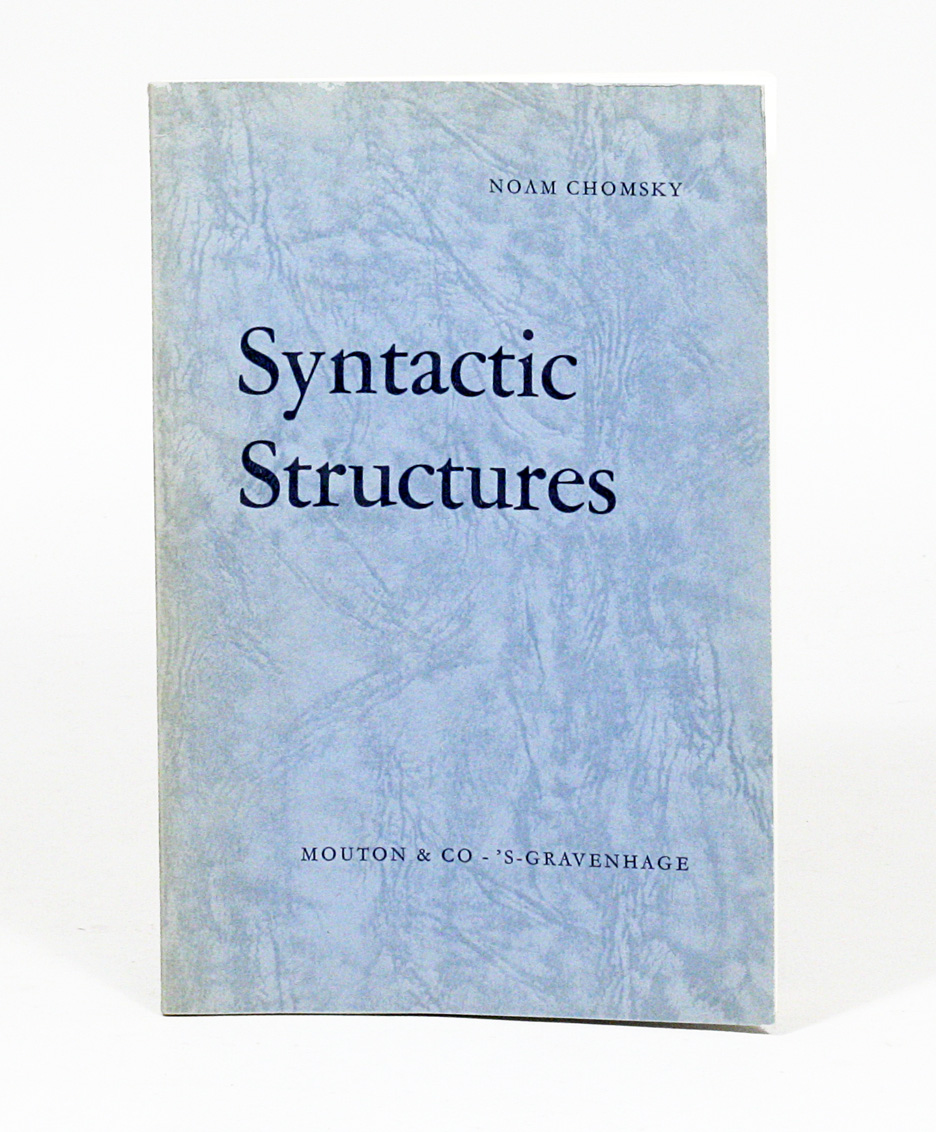
\includegraphics[scale=.2]{ss.jpg} 

Photo 4: His book
\subsection{Antiwar activism to Now}

Noam Chomsky published many articles outlining his feelings toward United States of America's involment in the Vietnam War[1]. All of these along with other accounts were all combined to create his very first political book which then led to many more. His protests and public disent led to his connection to the American New Left movement. Although during the beginning of this time period, he was relatively ignored by mainstream media.

Some things that Chomsky did to show his disent were: 
\begin{itemize}
\item Refuse to pay half of his taxes 
\item Publicly support students who refused the draft
\item Participate in an antiwar tech-in that was held outside of the Pentagon, which ultimately led to his arrest
\item Co-founded the antiwar group "RESIST"
\end{itemize}
He gave lots of lectures to student progressive groups and along with other professors, would offer undergraduate courses about conservative-dominated political science. 

Because of his massive disent, Chomsky was arrested many times and made it on the President Nixon's list of political opponents. Due to so many repercussions, his wife studied to become a Linguist in the case that he would become unemployed due to his belief. Thankfully, due to his reputation in science he had a protection on any administrative action concerning his beliefs.

During this time, he continued to gain popularity in his work of Linguistics -- receive multiple honorary doctorates. His debate with Michel foucault gave Noam Chomsky the conotation of a symbolic figurehead of analytic philosophy. He continued to publish works in linguistics, including the most famously known, "Studies on Semantics in Generative Grammar."

After the September 11 attacks on the United States, Chomsky gave plenty of interviews. He argued that the 'war' was not new but rather just a continuation of what was already United States' foreign policy from way back then. He widely disented the Iraq War and the ensuing 'war'.[1] He also took the time to visit Turkey and meet the man that was inprisoned for publishing Chomsky's work. While on the trip he also spoke on in favor of the Kurds' human rights [3]. 

Chomsky was not only well known for his work in Linguisitics but also a global figure for human rights and works to stop governments from becoming way too powerful for their own good. He currently works as a part-time professor in linguistics department at the University of Arizona. \newline

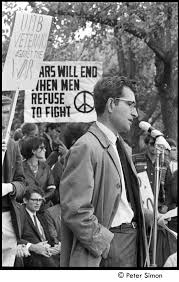
\includegraphics[scale=.5]{resist.jpg} 

Photo 5:Photo of his protest
\section{The Linguistic Theory}

\subsection{Background}
The Linguistic Theory is heavily influenced by Biolinguistics[5]. Biolinguistics is essentially the philosophy that states the principle of the structure of language are preset biologically in each persons mind, therefore it is inherited and passed on genetically[5]. Extending that principle he suggests that all humans share the same basic principle and linguistic set up, not impacted by sociocultural differences. He implicitely contradicted what Skinner had stated earlier in time saying that behavior is a learned aspect completely dependent on one's upbringing, rather he argues that it is inherited and has nothing to do with an organism or its environment [2].

Chomsky underlying states that language is unique to humans, which is what distinguishes US from other animal species. Thus, humans is the entire population not divided by country, race, or any other form of modern characteristics. What is interesting to note is that Chomsky's definition for language coincides with philisophical schoool of rationalism, while also defying with that of empiricism, which essentially states that knowledge comes from an outer influence [5]. 

\subsection{Influence of LT}

The use of his Linguistic Theory has brought up the aspects that there can be models (or actual grammars) that can decipher some characteristics of a certain language. These models can be used to see how languages may compare to one another and what could be said about how they are used differently. These syntactic similarites became known as 'transformations' which were unique in languages. Chomsky argued that languages were made up of two different parts, a deep and surface characteristic. Surface related to things that were audible and how to actually pronunciate words while deep referred to actual meanings and connotation toward what was being transferred. 

These models (grammars) were adopted and used in mathematical notation to show the relationship between both the surface and deep structures. Using this, there was the acception that linguistics could use math to create sentence composition in a unique language. 

\subsection{Chomsky Herarchy (Including: Regular, Context-Free, Context-Sensitive, Recursively Enumerable}

The presense of natural languages allowed for Chomsky to find a way to organize them into a form of sets that when connected to one another formed subsets of one another, this meant that those that were more complex became super sets. This organization ultimately became known as, "The Chomsky Heirarchy. " This organization is still very much in use and is incorporated into various language theories (including those of formal, theoretical computer science programming, compiler, and AUTOMATA). 

The way Chomsky Herachy grammars are written is in a certain format. Where nonterminals are the uppercase letters while terminal symbols are lowercase letters. Universally accepted the start symbol is the uppercase letter S. 

The general consensus on how to write these languages out are as follows:
\begin{itemize}
\item $w \rightarrow v$ where w,v = is a string that may contain a combination of terminal and nonterminal symbols. 
\item the way the two variables are formed and how the string is constructed is what influences into which classification the grammar falls into the Chomsky Heirarchy. 
\end{itemize}
This essential idea can be easily transferred to the various theories as stated above. For example, to show sentence structure we see that the following grammar is created using similar techiniques as computational programming.
Heres the list of nonterminals for sentence structure: 
\begin{itemize}
\item S = sentence 
\item N = nounphrase
\item V = verbphrase
\item VE = verb 
\item NO = noun
\item A = adjective
\end{itemize}
$S \rightarrow N \ V \newline 
N \rightarrow A \ N \newline 
N \rightarrow NO \newline
V \rightarrow VE \ N \newline
NO \rightarrow houses \| \ maps \newline 
VE \rightarrow run \| move \newline 
A \rightarrow amazing \| red $\newline 
Using this grammar we can easily create the sentence: "houses move maps" which is valid sentence in the english language. The levels of these grammars vary on complexity and how they are written. We have the simplest form of them in the shape of Regular which is your typical sentence format. Complex-free and complex-sensitive become a mix and match into create complex sentences for say. We allow recursion in these cases which makes them very powerful languages and can be used for various of things. 
\section{Conclusion}
Ultimately, Noam Chomsky did more than just provide a new way to look at Linguistics as a field. He revolutionized how any field can be interpretted and used widely and interdisciplinary. His field had implications ranging from English to Computers! He will really go down as one of the most brilliant minds the World has to offer. 
\section*{References}


[1] Glaser, John (November 18,2012). "It is not a war. It is murder". antiwar.com. Archived from the original on November 8, 2017.

[2] MacCorquodale, Kenneth (January 1970). "On Chomsky's review of Skinner's Verbal Behavior". Journal of the Experimental Analsis of Behavior. pg: 83-89.

[3] Milne, Seumas (November 7, 2009). "US foreign policy is straight out of the mafia". The Guardian

[4] "Noam Chomsky". MIT Linguistics Program. 2002.

[5] Ruiter, J. P. de; Levinson, Stephen C. (October 2010). "A biological infrastructure for comunication underlies the cultural evolution of languages". Behavioral and Brain Sciences. 

[6] Szabo, Zoltan Gendler (2010). "Chomsky, Noam Avram (1928-)". IN Shook, John R. (ed.). The Dictionary of Modern American Philosophers. Continuum.


\end{document}
